\documentclass{article}

\usepackage{graphicx}
\usepackage{amsfonts,amsmath,amssymb,amsthm}
\usepackage{url}
\usepackage[usenames]{color}






\newcommand{\G}{\mathcal{G}}


\newcommand{\ww}{{\bf w}}
\newcommand{\xx}{{\bf x}}
\newcommand{\yy}{{\bf y}}
\newcommand{\real}{\ensuremath{\mathbb{R}}}
\date{}
\title{Homework 3}
\author{(Inference and Representation) 
\\ Due October 15 on NYU Classes.  }
\usepackage{fullpage}
\begin{document}

\maketitle

\begin{enumerate}

\item {\bf Message passing on a tree. (From Murphy chapter 20)} 

Consider the DGM below which represents the following fictitious biological model. Each $G_i$ represents the genotype of a person: $G_i = 1$ if they have a healthy gene and $G_i = 2$ if they have an unhealthy gene. $G_2$ and $G_3$ may inherit the unhealthy gene from their parent $G_1$. $X_i\in \mathbb R$ is a continuous measure of blood pressure, which is low if you are healthy and high if you are unhealthy. We define the CPDs as follows

\begin{minipage}{0.6\textwidth}
\vspace{-30pt}
\begin{eqnarray*}
p(G_1) &=& [0.5, 0.5] \\
p(G_2|G_1) &=& \left( \begin{matrix} 0.9 & 0.1 \\ 0.1 & 0.9 \end{matrix} \right) \\
p(G_3|G_1) &=&  \left( \begin{matrix} 0.9 & 0.1 \\ 0.1 & 0.9 \end{matrix} \right) \\
p(X_i | G_i =1) &=& \mathcal N (X_i | \mu=50, \sigma^2 =10) \\
p(X_i | G_i =2) &=& \mathcal N (X_i | \mu=60, \sigma^2 =10) 
\end{eqnarray*}
\end{minipage}
\begin{minipage}{0.7\textwidth}
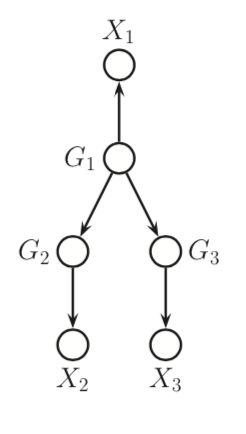
\includegraphics[width=0.22\textwidth]{fig_hw3}
\end{minipage}

\begin{enumerate}
\item Suppose you observe $X_2=50$ and $X_1$ is unobserved. What is the posterior belief on $G_1$ (i.e. $p(G_1|X_2=50)$?)
\item Now suppose you observe $X_2=50$ and $X_3=50$. What is $p(G_1| X_2, X_3)$? Explain your answer intuitively.
\item Now suppose $X_2=60$ and $X_3=60$. What is $p(G_1| X_2, X_3)$? Explain your answer intuitively.
\item Now suppose $X_2=50$ and $X_3=60$. What is $p(G_1| X_2, X_3)$? Explain your answer intuitively.
\end{enumerate}


\item  {\bf LDPC, (appeared in Joan Bruna's homework set).} 

We begin by designing algorithms for reliable communication in the presence of noise. We
focus on error correcting codes based on highly sparse, low density parity check (LDPC) matrices, and use the sum-product variant of the loopy belief propagation (BP) algorithm
to estimate partially corrupted message bits. For background information on LDPC codes, see Chap. 47 of MacKay's Information Theory, Inference, and Learning Algorithms, which
is freely available online: \url{http://www.inference.phy.cam.ac.uk/mackay/itila/}.

We consider rate 1/2 error correcting codes, which encode N message bits using a 2N-bit codeword. LDPC codes are specified by a $N \times 2N$ binary parity check matrix H,
whose columns correspond to codeword bits, and rows to parity check constraints. We define $H_{ij} = 1$ if parity check $i$ depends on codeword bit $j$, and $H_{ij} = 0$ otherwise. Valid codewords are those for which the sum of the bits connected to each parity check, as indicated by H, equals zero in modulo-2 addition (i.e., the number of "active" bits must be even). Equivalently, the modulo-2 product of the parity check matrix with the 2N-bit codeword vector must equal a N-bit vector of zeros. As illustrated in Figure \ref{fig:factor}, we can visualize these
parity check constraints via a corresponding factor graph. The parity check matrix H can then be thought of as an adjacency matrix, where rows correspond to factor (parity) nodes,
columns to variable (codeword bit) nodes, and ones to edges linking actors to variables.

\begin{figure}[t]
\centering
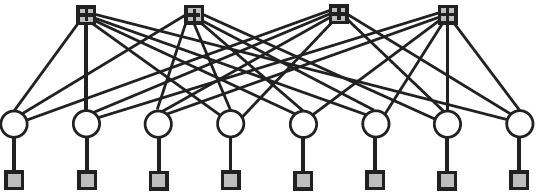
\includegraphics[width=2in]{brown_hw2}
\caption{A factor graph representation of a LDPC code linking four factor (parity constraint)
nodes to eight variable (message bit) nodes. The unary factors encode noisy observations of the
message bits from the output of some communications channel.}
\label{fig:factor}
\end{figure}

\begin{enumerate}
\item Implement code that, given an arbitrary parity check matrix H, constructs a corresponding factor graph. The parity check factors should evaluate to 1 if an even number of adjacent bits are active (equal 1), and 0 otherwise. Your factor graph representation should interface with your implementation of the sum-product algorithm from the previous problem. Define a small test case, and verify that your graphical model assigns zero probability to invalid codewords.
\item Load the $N = 128$-bit LDPC code using the Python library \path{pyldpc} (for a tutorial see \url {github.com/hichamjanati/pyldpc-tutos}).  To evaluate decoding
performance, we assume that the all-zeros codeword is sent, which always satisfies any set of parity checks. Using the random module, simulate the output of a binary symmetric
channel: each transmitted bit is flipped to its complement with error probability $\epsilon =0.05$, and equal to the transmitted bit otherwise. Define unary factors for each variable node
which equal $1-\epsilon$ if that bit equals the "received" bit at the channel output, and $\epsilon$ otherwise. Run the sum-product algorithm for 50 iterations of a parallel message update schedule, initializing by setting all variable-to-factor messages to be constant. After the final iteration, plot the estimated posterior probability that each codeword bit equals one.
If we decode by setting each bit to the maximum of its corresponding marginal, would we find the right codeword?
\item Repeat the experiment from part (b) for 10 random channel noise realizations with error probability $\epsilon= 0.06$. For each trial, run sum-product for 50 iterations. After each iteration, estimate the codeword by taking the maximum of each bit's marginal distribution, and evaluate the Hamming distance (number of differing bits) between the estimated and true (all-zeros) codeword. On a single plot, display 10 curves showing Hamming distance versus iteration for each Monte Carlo trial. Is BP a reliable decoding algorithm?
\item Repeat part (c) with two higher error probabilities, $\epsilon = 0.08$ and $\epsilon = 0.10$. Discuss any qualitative differences in the behavior of the loopy BP decoder.
\item For the LDPC codes we consider, we also define a corresponding $2N\times N$ generator matrix G. To encode an N-bit message vector we would like to transmit, we take the modulo-2 matrix product of the generator matrix with the message. The generator matrix has been constructed (via linear algebra over the  finite field GF(2)) such that this product always produces a valid 2N-bit codeword. Geometrically, its columns are chosen to span the null space of H. We use a systematic encoding, in which the first N codeword bits are simply copies of the message bits. The problems below use precomputed (G;H) pairs using the relevant functions in  \path{pyldpc}. Generate the $N = 1600$-bit LDPC code. Using this, we will replicate the visual decoding demonstration from MacKay's Fig. 47.5. Start by converting a $40\times 40$ binary image to a 1600-bit message vector. Encode the message using the  generator matrix $G$,
and add noise with error probability $\epsilon = 0.06$. For this input, plot images showing the output of the sum-product decoder after 0, 1, 2, 3, 5, 10, 20, and 30 iterations. The \%
operator may be useful for computing modulo-2 sums. You can use the numpy reshape function to easily convert between images and rasterized message vectors.
\item Repeat the previous part with a higher error probability of $\epsilon =0.10$, and discuss differences.
\end{enumerate}

\section*{Optional problems}

\item {\bf HMM with mixture model emissions, (appeared in Joan Bruna's homework set). \newline [10 points of extra credit]}
% From Berkeley, A_hw5_Fa11.tex
%\begin{center}{\bf \large  HMM with mixture model emissions}\end{center}

A common modification of the hidden Markov model involves using mixture models for the
emission probabilities $p(\yy_t | q_t)$, where $q_t$ refers to the state for time $t$ and $\yy_t$ to the observation for time $t$.

Suppose that ${\bf y}_t \in \real^n$ and that the emission distribution is given by a mixture of Gaussians for each value of the state. To be concrete, suppose that the $q_t$ can take $K$ discrete states and each mixture has $M$ components. Then,
\[
p({\bf y}_t \mid q_t) = \sum_{j=1}^M b_{q_t j}
\left(\frac{1}{(2\pi)^{\frac{n}{2}}|\Sigma_{q_t j}|^{\frac{1}{2}}}
\exp\left\{-\frac{1}{2}({\bf y}_t-\mu_{q_t j})^T\Sigma_{q_t j}^{-1}({\bf y}_t-\mu_{q_t j})
\right\}\right)
\]
where ${\bf b}_i \in [0,1]^M$ denotes the mixing weights for state $i$ ($\sum_{j=1}^M b_{ij} = 1$ for $i=1,\ldots K$), $\mu_{ij} \in  \real^n$ and $\Sigma_{ij} \in  \real^{n\times n}$.

Let $\pi \in \real^K$ be the probability distribution for the initial state $q_0$,
and $A \in \real^{K \times K}$ be the transition matrix of the $q_t$'s.
In this problem you will derive an EM algorithm for learning the parameters $\{ b_{ij}, \mu_{ij}, \Sigma_{ij} \}$ and $A, \pi$.

\begin{enumerate}
\item The EM algorithm is substantially simpler if you introduce auxiliary variables $z_t\in \{1, \ldots, M\}$ denoting which mixture component the $t$'th observation is drawn from.

Draw the graphical model for this modified HMM, identifying
  clearly the additional latent variables that are needed.
\item Write the expected complete log likelihood for the model
  and identify the expectations that you need to compute in the E
  step. {\em Show all steps of your derivation.}

\item Give an algorithm for computing the E step.

{\em Hint: Reduce the inference problem to something you know how to do, such as sum-product belief propagation in tree-structured pairwise MRFs.}

\item Write down the equations that implement the M step.
\end{enumerate}




\item {\bf Sum-product algorithm. From Brown University CS 242. \newline [10 points of extra credit]} 

We implement the sum-product variant of the belief propagation algorithm to compute marginals. To understand the details of the sum-product algorithm, we recommend Chapter 5 of Barber's ``Bayesian Reasoning and Machine Learning", as well as ``Factor Graphs and the Sum-Product Algorithm" by Kschischang, Frey, \& Loeliger, IEEE Trans. Information Theory 47, pp. 498-519, 2001.

You must write your own  implementation of the sum-product algorithm in Python.

We  provided code implementing a data structure to store the graph adjacency structure, and numeric potential tables, defining any discrete factor graph. We also provided code that explicitly builds a table containing the probabilities of all joint configurations of the variables in a factor graph, and sums these probabilities to compute the marginal
distribution of each variable. Such ``brute force" inference code is of course inefficient, and will only be computationally tractable for small models.

We recommend (but do not require) that you use these same data structures for your own implementation of the sum-product algorithm, by implementing \path{get_beliefs}. To gain intuition for the graph structure, examine the output of \path{make_debug_graph.ipynb}. Think of the code we provide as a starting point: you are welcome to create additional functions or data structures as needed. 

\begin{enumerate}
\item Implement the sum-product algorithm. Your code should support an arbitrary factor graph linking a collection of discrete random variables. Use a parallel message update schedule,
in which all factor-to-variable messages are updated given the current variable-to-factor messages, and then all variable-to-factor messages given the current factor-to-variable
messages. Initialize by setting the variable-to-factor messages to equal 1 for all states.
Be careful to normalize messages to avoid numerical underflow.


\item Consider the four-node, tree-structured factor graph illustrated in Figure \ref{fig:tree} with binary variables. Numeric values for the potential functions are defined in \path{make_debug_graph.ipynb}. Run your implementation of the sum-product algorithm on this graph, and report the marginal distributions it computes. 
\begin{figure}[h]
\centering
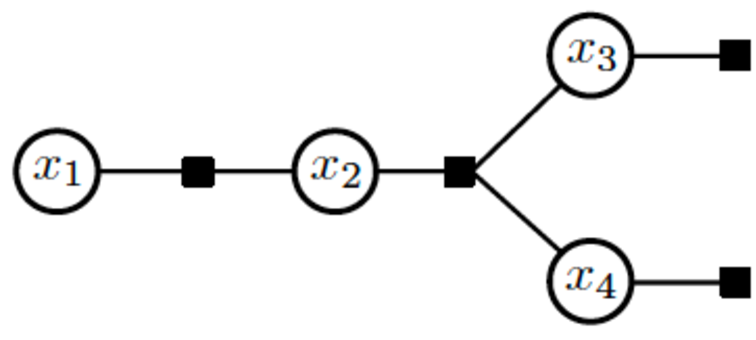
\includegraphics[width=2in]{brown_hw1}
\caption{A tree-structured factor graph in which four factors link four binary random variable.}
\label{fig:tree}
\end{figure}
\end {enumerate}

\end{enumerate}


\end{document}
